\section{Design di Dettaglio}
In questa sezione viene effettuata un'analisi del design di dettaglio, evidenziando aspetti interni ai componenti del
sistema, senza esplorare l'implementazione effettiva del codice.

\subsection{Design del Modello}
A partire dall'analisi dei requisiti funzionali del sistema, sono stati individuati gli aspetti fondamentali all'interno
del modello di gioco. Nello specifico, sono emerse due macro-categorie:
\begin{itemize}
    \item \textbf{Elementi Statici} - ovvero tutti gli aspetti che trascendono dalla singola partita.
    \item \textbf{Elementi Dinamici} - ovvero tutte le dinamiche che dipendono strettamente dalla partita in corso.
\end{itemize}

\subsubsection{Elementi Statici}
Dall'analisi dei requisiti, è emerso che le entità in gioco presentano tratti comuni e caratteristiche specifiche. In
particolare, un'entità deve possedere una posizione nello spazio di gioco e una dimensione; quindi, è stato modellato
un primo tratto comune \texttt{Entity} che rappresenta ogni oggetto sulla mappa, associandoci una posizione e una
dimensione. A partire da questo, sono state analizzate le entità da rappresentare, andando ad individuare una gerarchia
di caratteristiche atomiche che permettono di definire ogni sottotipo di \texttt{Entity} come combinazione di queste
ultime. Tali abilità, mostrate in figura \ref{fig:class-entity-hierarchy}, sono:
\begin{itemize}
    \item \texttt{Movement Ability} - aggiunge all'entità la capacità di cambiare la propria posizione in base alla
    propria velocità.
    \item \texttt{Track Following} - modifica la capacità di movimento limitando l'entità all'interno della traccia di
    gioco.
    \item \texttt{Popping Ability} - aggiunge all'entità una vita che può essere ridotta con un "pop" (chiamato così
    poiché concerne solamente i palloncini).
    \item \texttt{Sight Ability} - aggiunge all'entità la capacità di vedere altre entità all'interno del proprio campo
    visivo.
    \item \texttt{Enhanced Sight Ability} - aggiunge alla \texttt{Sight Ability} la capacità di vedere eventuali entità
    invisibili.
    \item \texttt{Rotation Ability} - aggiunge all'entità la capacità di ruotare su se stessa, modificando la propria
    direzione.
    \item \texttt{Shooting Ability} - aggiunge all'entità la capacità di sparare proiettili.
\end{itemize}

\begin{figure}[H]
    \centering
    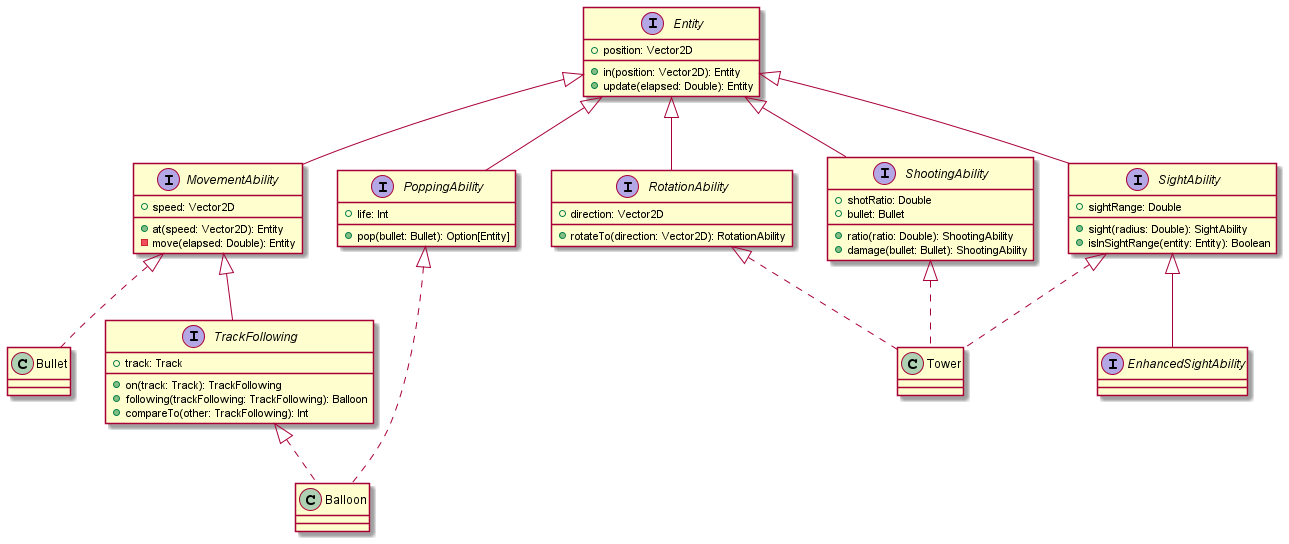
\includegraphics[width=\linewidth]{img/class-entity-hierarchy-extended}
    \caption{Diagramma delle classi della gerarchia di entità.}
    \label{fig:class-entity-abilities}
\end{figure}

Grazie a queste, è possibile esprimere le entità di gioco come segue:
\begin{itemize}
    \item Proiettile - entità con \texttt{Movement Ability} ed eventuale \texttt{Sight Ability} nel caso in cui possa
    esplodere, includendo nell'esplosione le entità all'interno del proprio campo visivo.
    \item Torre - entità con \texttt{Rotation Ability}, \texttt{Shooting Ability} e \texttt{Sight Ability}: infatti, le
    torri non possono muoversi, una volta istanziate, ma possono ruotare su se stesse e sparare proiettili verso i
    palloncini che rientrano nel loro campo visivo; eventualmente, la visione delle torri può essere potenziata con la
    \texttt{Enhanced Sight Ability}, per vedere palloncini invisibili.
    \item Palloncini - entità che si muove sulla traccia (\texttt{Track Following}) e che può essere scoppiata (
    \texttt{Popping Ability}).
\end{itemize}

Date le specifiche, è stato inoltre necessario definire un ulteriore sistema di riferimento spaziale che rappresenti la
mappa di gioco; è stata quindi realizzata una griglia sottostante all'interfaccia, che suddivide la mappa in celle per
riuscire a individuare punti a due coordinate nello spazio. Così facendo, è anche possibile rappresentare la traccia di
gioco come una sequenza ordinata di celle della griglia.

\subsubsection{Elementi Dinamici}
Inizialmente, è stato progettato il \texttt{Model} in modo che gestisse tutti gli aspetti dinamici del sistema.
Con l'espansione di tali elementi, il \texttt{Model} si è rivelato essere poco scalabile, oltre a doversi occupare di
aspetti logicamente distanti tra loro: quindi, è stato riprogettato per comunicare con degli appositi \textit{manager}
per ciascuno degli aspetti dinamici rilevati. Nello specifico, sono state riscontrate tre logiche fondamentali del
modello:
\begin{itemize}
    \item \textbf{Gestione delle entità in gioco} - ovvero tutte le interazioni con le entità che devono essere
    aggiornate nel corso della partita.
    \item \textbf{Generazione dei palloncini} - ovvero le politiche di \textit{spawn} dei palloncini, tenendo conto dei
    diversi tipi, della quantità, dell'ordine e del \textit{round} corrente.
    \item \textbf{Gestione dei dati di gioco} - ovvero il mantenimento delle statistiche di una partita, quali i punti
    vita, il denaro e la traccia di gioco.
\end{itemize}

Pertanto, il \texttt{Model} funge esclusivamente da \textit{relay} di messaggi, ridirezionandoli ai manager interessati:
tale design è fortemente ispirato al pattern \textbf{Facade} \cite{FacadePattern} e al tipico pattern di delegazione
spesso utilizzato in \textit{Akka}.

\begin{figure}[H]
    \centering
    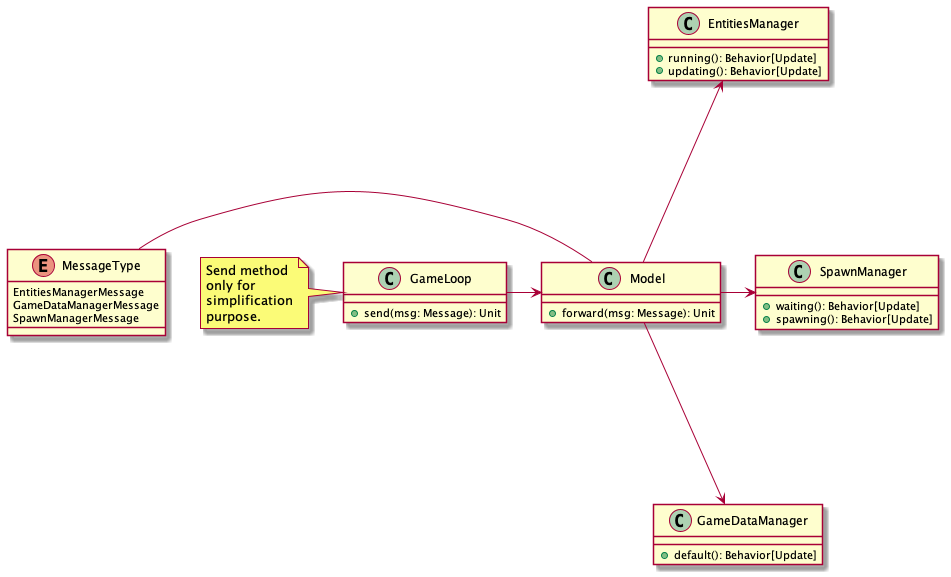
\includegraphics[width=.8\linewidth]{img/class-managers}
    \caption{Diagramma dei \textit{manager}.}
    \label{fig:managers}
\end{figure}

Nello specifico, il \textit{manager} delle entità è composto da due comportamenti principali:
\begin{itemize}
    \item \textbf{Running} - in cui vengono ricevuti e gestiti i messaggi provenienti da tutto il dominio escluse le
    entità, a partire dal \texttt{TickUpdate}, ossia il messaggio di aggiornamento del \texttt{GameLoop}.
    \item \textbf{Updating} - in cui attende che tutte le entità di gioco siano state aggiornate dai corrispettivi
    attori, per poi notificare il \texttt{GameLoop} e tornare al comportamento precedente.
\end{itemize}
Questa suddivisione è stata pensata per dare priorità ai messaggi in base allo stato di aggiornamento dei singoli attori
rappresentanti le entità: infatti, nel caso in cui il \textit{manager} ricevesse un messaggio mentre si trova nel
comportamento sbagliato, questi lo accoda per poi soddisfare la richiesta appena possibile.

\begin{figure}[H]
    \centering
    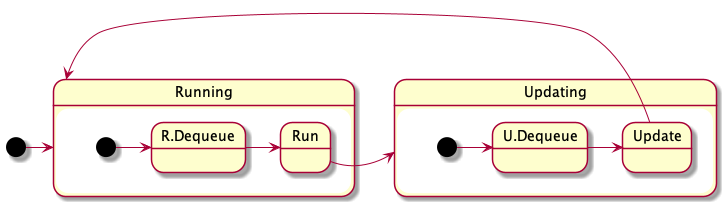
\includegraphics[width=\linewidth]{img/state-entities-manager}
    \caption{Diagramma di stato UML del \textit{manager} delle entità.}
    \label{fig:entities-manager}
\end{figure}

Per quanto riguarda il \textit{manager} della generazione dei palloncini, sono stati individuati due
macro-comportamenti:
\begin{itemize}
    \item \textbf{Waiting} - in cui attende un messaggio che comunica l'inizio del nuovo \textit{round}.
    \item \textbf{Spawning} - in cui effettua la generazione dei palloncini presenti all'interno del \textit{round}:
    tale comportamento si può ulteriormente suddividere in:
    \begin{itemize}
        \item \textbf{Spawning Round} - controlla se ci sono altre \textit{streak} di palloncini da generare: in caso
        positivo ne ordina la generazione, altrimenti ritorna in \texttt{Waiting}.
        \item \textbf{Spawning Streak} - genera i palloncini appartenenti ad una \textit{streak}.
        \item \textbf{Paused} - nel caso il gioco venga messo in pausa durante la generazione di palloncini, anche
        quest'ultima dovrebbe essere temporaneamente sospesa.
    \end{itemize}
\end{itemize}

\begin{figure}[H]
    \centering
    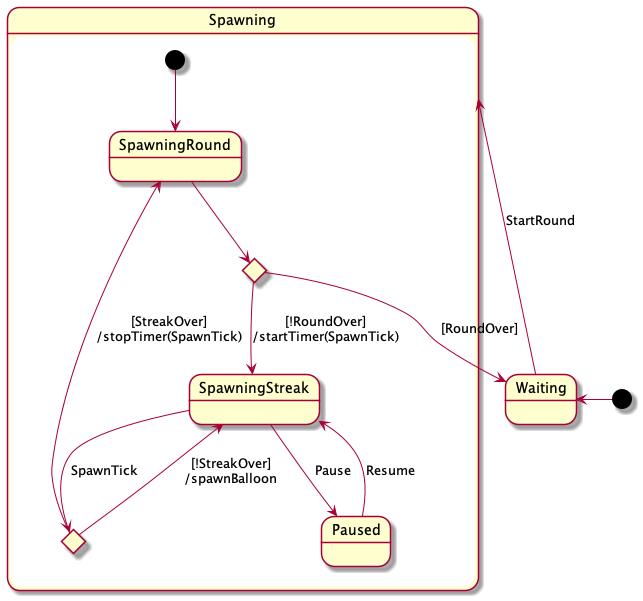
\includegraphics[width=.8\linewidth]{img/state-spawn-manager}
    \caption{Diagramma di stato UML del \textit{manager} della generazione dei palloncini.}
    \label{fig:spawn-manager}
\end{figure}

Infine, il \textit{manager} dei dati di gioco è semplicemente composto da un solo comportamento in cui modifica o
inoltra i dati quando richiesto.

\subsection{Design della View}
Come anticipato, per poter comunicare con il \texttt{Controller}, anche la \texttt{View} è stata progettata come un
attore. Vista la dipendenza del progetto da \textit{ScalaFX}, il suo compito principale è quello di agire su un insieme
di \textit{controller fxml} che contengono elementi grafici, e che permettono di modificare il contenuto
dell'interfaccia grafica. Data la complessità di queste componenti grafiche, l'attore della \texttt{View} è stato
modellato con un comportamento per ciascuna pagina del gioco:
\begin{itemize}
    \item inMenu, relativo al pagina del menù principale;
    \item inGame, relativo alla pagina di gioco;
    \item inSettings, relativo alla pagina delle impostazioni di gioco;
    \item inSavedTracks, relativo alla pagina in cui si possono vedere le tracce di partite già giocate.
\end{itemize}

La suddivisione (mostrata in figura \ref{fig:view-behaviors}) permette di ottenere accesso agli elementi grafici
solamente quando lo \textbf{stato} dell'attore lo concede e di semplificare l'implementazione dei \textit{controller}
non dovendone gestire l'interazione. Quindi, si potrebbe concludere che la \texttt{View} funga da \textbf{Facade}
\cite{FacadePattern}, con un'ulteriore fattore di modularizzazione dovuta all'introduzione dei comportamenti dell'attore.

\begin{figure}[H]
    \centering
    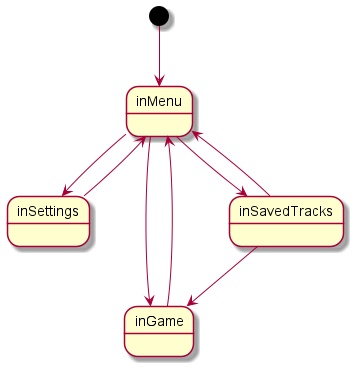
\includegraphics[width=.5\linewidth]{img/state-view-behaviors}
    \caption{Diagramma di stato UML dei comportamenti della \texttt{View}, che riflette la navigazione tra le pagine
    del sistema.}
    \label{fig:view-behaviors}
\end{figure}

Inoltre, per rispettare al meglio il pattern \textit{MVC}, il componente in discussione non ha alcun riferimento al
\texttt{Controller}, bensì viene sfruttato l'\textit{higher order} e vengono passati i metodi di invio e richiesta di
messaggi a ciascun \textit{controller fxml}, in modo da lasciare gli aspetti di input esclusivamente al
\texttt{Controller}.